\documentclass[Orbiter Developer Manual.tex]{subfiles}
\begin{document}

\section{Orbiter configuration files}
Configuration files allow the customisation of various aspects of the simulator. Configuration files have file extension .cfg. They are ASCII text files which can be edited with any text editor capable of writing plain text files (e.g. notepad).\\
Each line contains an item and its value, using the format

\begin{lstlisting}[language=OSFS]
<item> = <value>
\end{lstlisting}

\noindent
A semicolon starts a comment, continuing to the end of the line.\\
All configuration files, except the main configuration file (see "Main configuration file" in Orbiter User Manual), are located in a subdirectory tree defined by the ConfigDir entry in the main file, usually ".\textbackslash Config".

\subsection{Planetary systems}
\label{ssec:planetery_sys}
Planetary systems contain stars, planets and moons. Each planetary system requires at least one star. Stars, planets and moons are defined in the planetary system's configuration file\\
\indent .\textbackslash Config\textbackslash <\textit{Solsys-name}>.cfg\\
Orbiter can support multiple planetary systems, but only one per scenario. The planetary system to be used by a scenario is referenced in the scenario file (see section \ref{sec:scn_files}).

\subsubsection*{General parameters}

%\begin{table}[H]
	%\centering
	\begin{longtable}{ |p{0.25\textwidth}|p{0.09\textwidth}|p{0.58\textwidth}| }
	\hline\rule{0pt}{2ex}
	\textbf{Item} & \textbf{Type} & \textbf{Description}\\
	\hline\rule{0pt}{2ex}
	Name & String & A name for the planetary system\\
	\hline\rule{0pt}{2ex}
	MarkerPath & String & Directory path containing celestial marker lists for the planetary system (see section \ref{ssec:custom_markers}). Default: .\textbackslash Config\textbackslash <\textit{Solsys-name}>\textbackslash Marker\textbackslash \\
	\hline
	\end{longtable}
%\end{table}

\subsubsection*{Object list}
The object list defines the celestial bodies populating the planetary system and their hierarchy.\\
\\
\textbf{Star entries:}

\begin{lstlisting}[language=OSFS]
Star<i> = <Name>
\end{lstlisting}

\noindent
where <\textit{i}> is an index running from 1 upward. (Note: planetary systems with more than one central star are not currently supported).\\
\\
\textbf{Planet entries:}

\begin{lstlisting}[language=OSFS]
Planet<i> = <Name>
\end{lstlisting}

\noindent
where <\textit{i}> is an index running from 1 upward.\\
\\
\textbf{Moon entries:}

\begin{lstlisting}[language=OSFS]
<Planet>:Moon<i> = <Name>
\end{lstlisting}

\noindent
where <\textit{Planet}> is the name of a planet defined before, and <\textit{i}> is an index enumerating the moons of this planet, running from 1 upward.\\
\\
\textbf{Example:}

\begin{lstlisting}[language=OSFS]
Star1 = Sun
Planet1 = Mercury
Planet2 = Venus
Planet3 = Earth
Earth:Moon1 = Moon
Planet4 = Mars
Mars:Moon1 = Phobos
Mars:Moon2 = Deimos
\end{lstlisting}


\subsection{Planets}
\label{ssec:planets}
Adding a new celestial body (planet or moon) to a planetary system requires the following steps:

\begin{itemize}
\item Add an entry for the body in the planetary system configuration file (see section \ref{ssec:planetery_sys}).
\item Create a configuration file for the planet, defining its orbital, physical and visual parameters, located in .\textbackslash Config\textbackslash <\textit{Planet-name}>.cfg, for example, Config\textbackslash Earth.cfg. The configuration entries are described below.
\item Create the required surface texture maps, and optionally elevation, night light, water mask, cloud layer and feature label maps. See section \ref{ssec:planetery_tex} for details.
\item Optionally, create configuration files for surface bases in .\textbackslash Config\textbackslash <\textit{Planet-name}>\textbackslash Base and reference them in the planet configuration file. See section \ref{ssec:surface_bases} for details on surface base definitions.
\item Optionally, compile a DLL module for the planet for ephemeris calculations and atmospheric parameter computation. See the Orbiter sources for examples, e.g., the Src\textbackslash Celbody\textbackslash Vsop87 project.
\item Optionally, create polyline definitions for coastlines (.\textbackslash Config\textbackslash <\textit{Planet-name}>\textbackslash Data\textbackslash coast.vec) and/or topography (.\textbackslash Config\textbackslash <\textit{Planet-name}>\textbackslash Data\textbackslash contour.vec) to be used in scalable map displays. See .\textbackslash Config\textbackslash Earth\textbackslash Data\textbackslash coast.vec for an example.
\end{itemize}

\noindent
The components of the planet configuration file are listed below. An example for a configuration file can be found in .\textbackslash Config\textbackslash Earth.cfg.

\subsubsection*{General parameters}
%\begin{table}[H]
	%\centering
	\begin{longtable}{ |p{0.25\textwidth}|p{0.09\textwidth}|p{0.58\textwidth}| }
	\hline\rule{0pt}{2ex}
	\textbf{Item} & \textbf{Type} & \textbf{Description}\\
	\hline\rule{0pt}{2ex}
	Name & String & Planet name\\
	\hline\rule{0pt}{2ex}
	Module & String & Name of a dynamic link library performing calculations for the planet. Default: none\\
	\hline\rule{0pt}{2ex}
	ErrorLimit & Float & Max. rel. error for position/velocity calculations (only used if the module supports precision adjustment)\\
	\hline\rule{0pt}{2ex}
	EllipticOrbit & Bool & If TRUE, use analytic 2-body solution for planet position/velocity calculation, otherwise update dynamically (ignored if module supports position/velocity calculation)\\
	\hline\rule{0pt}{2ex}
	HasElements & Bool & If TRUE, the initial position/velocity is calculated from the provided set of orbital elements, otherwise from an explicit position/velocity pair (ignored if the module supports position/velocity calculation)\\
	\hline\rule{0pt}{2ex}
	InitPos & Vec3 & TODO (legacy?)\\
	\hline\rule{0pt}{2ex}
	InitVel & Vec3 & TODO (legacy?)\\
	\hline
	\end{longtable}
%\end{table}

\noindent
Notes:\\
If the module calculates the planet position and velocity from a numerical series expansion solution, the value of ErrorLimit affects the number of terms used for the calculation. A lower value increases the number of terms required to achieve that limit, and thus increases calculation time. The valid range for ErrorLimit depends on the module, but is typically 10$^{-3}$ $\leq$ ErrorLimit $\leq$ 10$^{-8}$.


\subsubsection*{Orbital parameters}
Ignored if a module is active that supports position/velocity calculation or if HasElements = FALSE.

%\begin{table}[H]
	%\centering
	\begin{longtable}{ |p{0.25\textwidth}|p{0.09\textwidth}|p{0.58\textwidth}| }
	\hline\rule{0pt}{2ex}
	\textbf{Item} & \textbf{Type} & \textbf{Description}\\
	\hline\rule{0pt}{2ex}
	Epoch & Float & Orbital element reference epoch (e.g. 2000)\\
	\hline\rule{0pt}{2ex}
	ElReference & Flag & Orbit reference frame (ParentEquator or Ecliptic). Default: Ecliptic\\
	\hline\rule{0pt}{2ex}
	SemiMajorAxis & Float & Orbit semi-major axis \textit{a} [m]\\
	\hline\rule{0pt}{2ex}
	Eccentricity & Float & Orbit eccentricity \textit{e}.\\
	\hline\rule{0pt}{2ex}
	Inclination & Float & Orbit inclination against reference frame \textit{i} [rad]\\
	\hline\rule{0pt}{2ex}
	LongAscNode & Float & Longitude of ascending node $\Omega$ [rad]\\
	\hline\rule{0pt}{2ex}
	LongPerihelion & Float & Longitude of periapsis $\overline{\omega}$ [rad]\\
	\hline\rule{0pt}{2ex}
	MeanLongitude & Float & Mean longitude \textit{l} at epoch [rad]\\
	\hline
	\end{longtable}
%\end{table}


\subsubsection*{Physical parameters}
%\begin{table}[H]
	%\centering
	\begin{longtable}{ |p{0.25\textwidth}|p{0.09\textwidth}|p{0.58\textwidth}| }
	\hline\rule{0pt}{2ex}
	\textbf{Item} & \textbf{Type} & \textbf{Description}\\
	\hline\rule{0pt}{2ex}
	Mass & Float & Planet mass [kg]\\
	\hline\rule{0pt}{2ex}
	Size & Float & Mean planet radius [m]\\
	\hline\rule{0pt}{2ex}
	JCoeff & List & Coefficients Jn of the harmonic expansion of planet ellipsoid shape, starting with J2\\
	\hline
	\end{longtable}
%\end{table}


\subsubsection*{Rotation and precession elements}
See also "Planetary axis precession" in Orbiter Technical Reference.

%\begin{table}[H]
	%\centering
	\begin{longtable}{ |p{0.25\textwidth}|p{0.09\textwidth}|p{0.58\textwidth}| }
	\hline\rule{0pt}{2ex}
	\textbf{Item} & \textbf{Type} & \textbf{Description}\\
	\hline\rule{0pt}{2ex}
	SidRotPeriod & Float & Sidereal rotation period [s]. Default: infinite\\
	\hline\rule{0pt}{2ex}
	SidRotOffset & Float & Rotation at epoch [rad]. Default: 0\\
	\hline\rule{0pt}{2ex}
	Obliquity & Float & Obliquity of axis: angle between planet axis and precession reference axis [rad]. Default: 0\\
	\hline\rule{0pt}{2ex}
	LAN & Float & Longitude of ascending node of equatorial plane [rad]. Default: 0\\
	\hline\rule{0pt}{2ex}
	LAN\_MJD & Float & Reference data for LAN [MJD]. Default: 51544.5\\
	\hline\rule{0pt}{2ex}
	PrecessionPeriod & Float & Period of precession of axis [days]. Default: infinite\\
	\hline\rule{0pt}{2ex}
	PrecessionObliquity & Float & Obliquity of precession reference axis with respect to ecliptic north pole at J2000 [rad]. Default: 0\\
	\hline\rule{0pt}{2ex}
	PrecessionLAN & Float & Longitude of ascending node of precession reference plane [rad]. Default: 0\\
	\hline
	\end{longtable}
%\end{table}


\subsubsection*{Gravity model parameters}
Gravity model only used it all parameters are present. See also "Nonspherical gravitational field perturbations" in Orbiter Technical Reference.

%\begin{table}[H]
	%\centering
	\begin{longtable}{ |p{0.25\textwidth}|p{0.09\textwidth}|p{0.58\textwidth}| }
	\hline\rule{0pt}{2ex}
	\textbf{Item} & \textbf{Type} & \textbf{Description}\\
	\hline\rule{0pt}{2ex}
	GravModelPath & String & Gravity model file name (with extension), relative to ".\textbackslash GravityModels" folder.\\
	\hline\rule{0pt}{2ex}
	GravCoeffCutoff & Int & Gravity model coefficient cutoff.\\
	\hline
	\end{longtable}
%\end{table}


\subsubsection*{Terrain parameters}
%\begin{table}[H]
	%\centering
	\begin{longtable}{ |p{0.25\textwidth}|p{0.09\textwidth}|p{0.58\textwidth}| }
	\hline\rule{0pt}{2ex}
	\textbf{Item} & \textbf{Type} & \textbf{Description}\\
	\hline\rule{0pt}{2ex}
	TileFormat & Int & 1 = legacy, 2 = 2016 format. Default: 1\\
	\hline\rule{0pt}{2ex}
	MaxPatchResolution & Int & Max. resolution level for surface texture maps (1-21)\\
	\hline\rule{0pt}{2ex}
	MaxElevation & Float & Max. surface elevation rel. to planet mean radius [m].\\
	\hline\rule{0pt}{2ex}
	MinElevation & Float & Min. surface elevation rel. to planet mean radius [m]. Used to adjust lower edge of rendered horizon.\\
	\hline\rule{0pt}{2ex}
	ElevationResolution & Float & Target resolution of elevation data [m].\\
	\hline\rule{0pt}{2ex}
	HorizonExcess & Float & Specifies how far beyond the sphere-based horizon to render tiles (to avoid mountains to disappear) [planet radius]. Default: 0.002\\
	\hline
	\end{longtable}
%\end{table}


\subsubsection*{Atmospheric parameters}
Only required if the planet defines an atmosphere.

%\begin{table}[H]
	%\centering
	\begin{longtable}{ |p{0.25\textwidth}|p{0.09\textwidth}|p{0.58\textwidth}| }
	\hline\rule{0pt}{2ex}
	\textbf{Item} & \textbf{Type} & \textbf{Description}\\
	\hline\rule{0pt}{2ex}
	AtmPressure0 & Float & (Mean) atmospheric pressure at zero altitude (reference radius) [Pa]\\
	\hline\rule{0pt}{2ex}
	AtmDensity0 & Float & (Mean) atmospheric density at zero altitude [kg/m$^{3}$]\\
	\hline\rule{0pt}{2ex}
	AtmGasConstant & Float & Specific gas constant [J K$^{-1}$ kg$^{-1}$]. Default: 286.91 (Earth value)\\
	\hline\rule{0pt}{2ex}
	AtmGamma & Float & Ratio of specific heats $c_{p}$/$c_{v}$. Default: 1.4 (Earth value)\\
	\hline\rule{0pt}{2ex}
	AtmColor0 & Vec3 & RGB triplet for atmospheric colour at ground level (0-1 each)\\
	\hline\rule{0pt}{2ex}
	AtmAltLimit & Float & Altitude limit beyond which atmospheric effects can be ignored [m]\\
	\hline\rule{0pt}{2ex}
	AtmHazeExtent & Float & Width parameter for extent of horizon haze rendering. Range: 0 (thinnest) to 1 (widest). Default: 0.1\\
	\hline\rule{0pt}{2ex}
	AtmHazeShift & Float & Shift the reference altitude of the haze base line (in units of planet radius). Can be used to adjust haze altitude to a cloud layer. Default: 0 (align with surface horizon). Shift is not applied if camera is below cloud layer.\\
	\hline\rule{0pt}{2ex}
	AtmHazeDensity & Float & Modify the density at which the horizon haze is rendered (basic density is calculated from atmospheric density). Default: 1.0\\
	\hline\rule{0pt}{2ex}
	AtmHazeColor & Vec3 & RGB triplet for horizon haze colour (0-1 each). Default: use AtmColor0 values.\\
	\hline\rule{0pt}{2ex}
	AtmFogColor & Vec3 & RGB triplet for distance fog colour (0-1 each).\\
	\hline\rule{0pt}{2ex}
	AtmFogParam & Vec3 & Value 1: fog density at surface level\newline
	Value 2: fog density at reference altitude\newline
	Value 3: reference altitude [m]\\
	\hline\rule{0pt}{2ex}
	AtmTintColor & Vec3 & RGB triplet for additive colour component (0-1 each) added to surface rendering at high altitude\\
	\hline\rule{0pt}{2ex}
	AtmAttenuationAlt & Float & Altitude limit for calculation of light attenuation on vessels [m].\\
	\hline\rule{0pt}{2ex}
	AtmHorizonAlt & Float & Altitude scale for horizon haze rendering [m]. Default: 0.01 of planet radius.\\
	\hline\rule{0pt}{2ex}
	ShadowDepth & Float & Depth ("blackness") of object shadows (0-1, where 0 = black, 1 = no shadows). Default: exp(-$\rho_{0}$/2), where $\rho_{0}$ is atmospheric density at the surface. This option is only used when stencil buffering is enabled, otherwise shadows are always black.\\
	\hline
	\end{longtable}
%\end{table}


\subsubsection*{Cloud parameters}
Only required if the planet defines a cloud layer.

%\begin{table}[H]
	%\centering
	\begin{longtable}{ |p{0.25\textwidth}|p{0.09\textwidth}|p{0.58\textwidth}| }
	\hline\rule{0pt}{2ex}
	\textbf{Item} & \textbf{Type} & \textbf{Description}\\
	\hline\rule{0pt}{2ex}
	CloudFormat & Int & 1 = legacy, 2 = 2016 format. Default: 1\\
	\hline\rule{0pt}{2ex}
	MinCloudResolution & Int & Min. resolution at which clouds are rendered as a separate layer (1-8)\\
	\hline\rule{0pt}{2ex}
	MaxCloudResolution & Int & Max. cloud resolution level (MinCloudResolution - 19)\\
	\hline\rule{0pt}{2ex}
	CloudAlt & Float & Altitude of cloud layer [m]\\
	\hline\rule{0pt}{2ex}
	CloudShadowDepth & Float & Depth ("blackness") of cloud shadows on the ground (0-1, where 0 = black, 1 = don't render shadows). Default: 1\\
	\hline\rule{0pt}{2ex}
	CloudRotPeriod & Float & Rotation period of cloud layer against surface [s]. Default: 0 (static cloud layer)\\
	\hline\rule{0pt}{2ex}
	CloudMicrotextureAlt & Float Float & Altitude range for cloud microtexturing.\newline
	Value 1: altitude at which full microtexturing is applied.\newline
	Value 2: altitude at which microtexture starts to kick in\newline
	Value 1 $\geq$ 0 and Value 2 > Value 1 is required. Default: no microtexture\\
	\hline\rule{0pt}{2ex}
	BrightenClouds & Bool & Use a brighter cloud rendering algorithm\\
	\hline
	\end{longtable}
%\end{table}


\subsubsection*{Visualisation parameters}
%\begin{table}[H]
	%\centering
	\begin{longtable}{ |p{0.25\textwidth}|p{0.09\textwidth}|p{0.58\textwidth}| }
	\hline\rule{0pt}{2ex}
	\textbf{Item} & \textbf{Type} & \textbf{Description}\\
	\hline\rule{0pt}{2ex}
	SpecularRipple & Bool & If TRUE, and if "Specular ripples" option is enabled in the Launchpad dialog, specularly reflecting surfaces use a "water ripple" microtexture. Default: FALSE\\
	\hline\rule{0pt}{2ex}
	AlbedoRGB & Vec3 & Albedo for dot representation (when far away). Default: (1, 1, 1)\\
	\hline\rule{0pt}{2ex}
	BBExcess & Float & Specifies how much to inflate the bounding box (1 = double each side)\\
	\hline
	\end{longtable}
%\end{table}


\subsubsection*{Planetary ring parameters}
Only required if the planet defines a ring system. All parameters needed.

%\begin{table}[H]
	%\centering
	\begin{longtable}{ |p{0.25\textwidth}|p{0.09\textwidth}|p{0.58\textwidth}| }
	\hline\rule{0pt}{2ex}
	\textbf{Item} & \textbf{Type} & \textbf{Description}\\
	\hline\rule{0pt}{2ex}
	RingMaxRadius & Float & Max. ring diamenter [planet radius].\\
	\hline\rule{0pt}{2ex}
	RingMinRadius & Float & Min. ring diamenter [planet radius].\\
	\hline
	\end{longtable}
%\end{table}


\subsubsection*{Surface marker parameters}
%\begin{table}[H]
	%\centering
	\begin{longtable}{ |p{0.25\textwidth}|p{0.09\textwidth}|p{0.58\textwidth}| }
	\hline\rule{0pt}{2ex}
	\textbf{Item} & \textbf{Type} & \textbf{Description}\\
	\hline\rule{0pt}{2ex}
	LabelFormat & Int & 1 = legacy surface markers (see section \ref{ssec:custom_markers}), 2 = quadtree-based marker definitions, see section \ref{sssec:label_tile_format}, uses tiles. Default: 1\\
	\hline\rule{0pt}{2ex}
	MarkerPath & String & Directory path to the legacy surface marker files for the planet. Default: .\textbackslash Config\textbackslash <\textit{Planet-name}>\textbackslash Marker\textbackslash \\
	\hline
	\end{longtable}
%\end{table}


\subsubsection*{Surface bases (optional)}
This is a list containing the names and locations of surface landing installations ("spaceports"). Each entry in the list must be accompanied by a configuration file for the corresponding surface base (see section \ref{ssec:surface_bases}).

\begin{lstlisting}[language=OSFS]
BEGIN_SURFBASE
	<base list>
END_SURFBASE
\end{lstlisting}

\noindent
Base list entries have the following format:

\begin{lstlisting}[language=OSFS]
<name> <lng> <lat>
\end{lstlisting}

\noindent
where

\begin{itemize}
\item <\textit{name}> $\Rightarrow$ Name identifying the base config file (<\textit{name}>.cfg). The actual base name as it appears in Orbiter is given by the NAME tag in the base config file.
\item <\textit{lng}> <\textit{lat}> $\Rightarrow$ Base centre position in equatorial coordinates [deg]
\end{itemize}


\subsubsection*{Ground-based observer sites (optional)}
This is a list containing the pre-defined locations for ground-based observers (launch cameras, spectators, etc.) which can be selected in the Camera dialog. The format of the list is

\begin{lstlisting}[language=OSFS]
BEGIN_OBSERVER
	<observer list>
END_OBSERVER
\end{lstlisting}

\noindent
List entries have the following format:

\begin{lstlisting}[language=OSFS]
<site>:<spot>: <lng> <lat> <alt>
\end{lstlisting}

\noindent
where

\begin{itemize}
\item <\textit{site}> $\Rightarrow$ Name identifying the site (e.g. KSC)
\item <\textit{spot}> $\Rightarrow$ The particular location at the site (e.g. Launch pad 39A)
\item <\textit{lng}> <\textit{lat}> $\Rightarrow$ Observer position in equatorial coordinates [deg]
\item <\textit{alt}> $\Rightarrow$ observer altitude (> 0) [m]
\end{itemize}

\noindent
The easiest way to find the coordinates for a new observer spot is to open the Camera dialog (\Ctrl+\keystroke{F1}), and select a nearby location under the Ground tab. Then move the camera to the new spot using \Ctrl\DArrow\UArrow\RArrow\LArrow and \keystroke{PageUp}\keystroke{PageDown}. The coordinates are displayed in the dialog and can be directly copied into the configuration file.


\subsubsection*{Navbeacon transmitter list (optional)}
This is a list containing the specs of all navigation radio transmitters on the planet surface except for those directly associated with a spaceport, which are defined in the base definition file (see section \ref{ssec:surface_bases}). The list format is as follows:

\begin{lstlisting}[language=OSFS]
BEGIN_NAVBEACON
	<NAV list>
END_NAVBEACON
\end{lstlisting}

\noindent
List entries defining individual transmitters have the following format:

\begin{lstlisting}[language=OSFS]
<type> <id> <lng> <lat> <freq> [<range>]
\end{lstlisting}

\noindent
where

\begin{itemize}
\item <\textit{type}> $\Rightarrow$ transmitter type, currently supported: VOR
\item <\textit{id}> $\Rightarrow$ identifier code (up to 4 characters)
\item <\textit{lng}> <\textit{lat}> $\Rightarrow$ transmitter position in equatorial coordinates [deg]
\item <\textit{freq}> $\Rightarrow$ transmitter frequency [MHz]
\item <\textit{range}> $\Rightarrow$ transmitter range [m]. Default: 500 000
\end{itemize}


\subsection{Surface bases}
\label{ssec:surface_bases}
Surface bases (or "spaceports") are launch and landing sites on the surface of planets or moons, usually equipped with launchpads and/or runways, for vertical and horizontal take-off and/or landing. Each surface base is defined in its own configuration file. When Orbiter loads a planet configuration, it scans all surface base definitions and creates the corresponding bases.

\subsubsection*{Base definition file}
Each surface base must be defined with a base configuration file. By default, this will be located in\\
\indent .\textbackslash Config\textbackslash <\textit{Planet-name}>\textbackslash Base\textbackslash <\textit{Base-name}>.cfg\\
where <\textit{Planet-name}> is the name of the celestial body the base is located on, and <\textit{Base-name}> is the name of the surface base. Different locations for the base folder can be defined, for example to allow selective base loading (see \textit{Linking surface bases to planets} below).\\
The format of the surface base definition file is as follows:

\begin{lstlisting}[language=OSFS]
BASE-V2.0
NAME = <Base-name>
LOCATION = <lng> <lat>
SIZE = <size>
OBJECTSIZE = <osize>
MAPOBJECTSTOSPHERE = [TRUE|FALSE]

BEGIN_NAVBEACON
	<NAV list>
END_NAVBEACON

BEGIN_OBJECTLIST
	<Object list>
END_OBJECTLIST

BEGIN_SURFTILELIST
	<Surface tile list>
END_SURFTILELIST
\end{lstlisting}

\noindent
where

\begin{itemize}
\item BASE-V2.0 $\Rightarrow$ Format identifier (must be placed in the first line of the file). This item is optional if the base is defined directly in the planet's base list.
\item NAME = <\textit{Base-name}> $\Rightarrow$ Logical name of the base as it will be displayed by Orbiter. Doesn't need correspond to the base file name.
\item LOCATION = <\textit{lng}> <\textit{lat}> $\Rightarrow$ The position of the base reference point on the planet surface, where <\textit{lng}> [deg] is longitude (< 0 for west, > 0 for east), and <\textit{lat}> [deg] is latitude (< 0 for south, > 0 for north). This item is optional if the base is defined directly in the planet's base list.
\item SIZE = <\textit{size}> $\Rightarrow$ Specifies the size of the base's footprint on the planet surface (defined as its mean radius [m]. This parameter determines the camera distance at which Orbiter will start rendering the base.
\item OBJECTSIZE = <\textit{osize}> $\Rightarrow$ Defines the "typical" size of individual base objects (buildings, etc.). In addition to the SIZE parameter, this value is used by Orbiter to fine-tune the rendering of base objects. Objects will not be rendered if the apparent size of an object of size <\textit{osize}> located at the base reference point, would be smaller than 1 pixel. The default value for <\textit{osize}> is 100.0.
\item MAPOBJECTSTOSPHERE = [TRUE|FALSE] $\Rightarrow$ If TRUE, the altitude of objects in the object list will be adjusted automatically to map them from a flat plane onto a spherical planet surface. So for example, a building defined with altitude 0 will be rendered at altitude 0 relative to the planet's reference sphere. If FALSE, elevation 0 maps onto the flat plane tangential to the base reference point (and therefore to a point above the reference sphere for any objects not located at the reference point). Default: FALSE\\
Note: Currently this function is only implemented for a limited number of base object types.
\item <\textit{NAV list}> $\Rightarrow$ Contains a list of navigation radio transmitters associated with the base. The format of the list is identical to the <\textit{NAV list}> in the planet configuration file (see section \ref{ssec:planets}).
\item <\textit{Object list}> $\Rightarrow$ Contains a list of objects which make up the visual elements of the base. See next section for details.
\item <\textit{Surface tile list}> $\Rightarrow$ This list is deprecated and is only retained for backward compatibility of old planet definitions. See section \ref{ssec:planetery_tex} for details on how to define surface textures for new planet definitions, including high-resolution patches around surface bases.
\end{itemize}


\subsubsection*{Linking surface bases to planets}
After creating the base configuration file, it must be referenced by a planet to instantiate the base. There are several ways to make Orbiter read a surface base definition:

\begin{itemize}
\item Place the base configuration file in the default base configuration folder for the planet. By default, Orbiter scans the folder .\textbackslash Config\textbackslash <\textit{Planet-name}>\textbackslash Base for base definitions. The default folder is scanned only if the planet doesn't explicitly define a base list (see below).
\item To make Orbiter scan different folders, create a surface base list in the planet's configuration file, enclosed by BEGIN\_SURFBASE and END\_SURFBASE tags (see section \ref{ssec:planets}). In this list, specify the new surface base directory with the line 'DIR <\textit{folder}>', where <\textit{folder}> is the path to the folder containing the base configurations (relative to the Config folder). Multiple folders can be specified. If the same base is defined in more than one of the scanned folders, only the first is used. This allows to replace base definitions without having to delete the original configuration file. Example:

\begin{lstlisting}[language=OSFS]
BEGIN_SURFBASE
	DIR Earth\MyBases
	DIR Earth\MoreBases
END_SURFBASE
\end{lstlisting}

\noindent
If the surface base list exists in a planet's configuration file, the default base configuration folder is not scanned, unless it is explicitly listed.
\item Base references can be placed directly into the base list, using the following format:\\

\begin{lstlisting}[language=OSFS]
<Base-name>:<lng> <lat>
\end{lstlisting}

\noindent
where <\textit{Base-name}> is the name of the base configuration file, .\textbackslash Config\textbackslash <\textit{Base-name}>.cfg, and <\textit{lng}> and <\textit{lat}> are the equatorial coordinates (longitude and latitude) of the base reference point in degrees. This position supersedes the one defined in the base configuration file, so the same base can be used in multiple locations. When using this format, the base configuration file must be located in the .\textbackslash Config folder.
\end{itemize}


\subsubsection*{Selective loading of bases}
To provide more control over the loading of surface bases in a specific simulation scenario, two conditional flags can be set with a DIR entry in the base list:

\begin{itemize}
\item Specify a time interval with the PERIOD parameter. The corresponding directory is only scanned if the scenario start date is inside this interval. This allows to add or replace surface bases only during specific time periods, for example to set up Kennedy Space Center for the Apollo lunar missions. Syntax:

\begin{lstlisting}[language=OSFS]
DIR <folder> PERIOD <MJD0> <MJD1>
\end{lstlisting}

\noindent
where <\textit{MJD0}> and <\textit{MJD1}> are the start and end dates of the period over which the base folder is scanned, in MJD (Modified Julian Date) format [days]. Either can be set to '-' to disable the limit at one end.
\item Specify a scenario context with the CONTEXT parameter. The corresponding directory is scanned only if the scenario specifies the same context string in its environment context entry (see section \ref{sec:scn_files}). This allows to add or replace bases only within a defined set of scenarios. Syntax:

\begin{lstlisting}[language=OSFS]
DIR <folder> CONTEXT <string>
\end{lstlisting}

\noindent
where <\textit{string}> is the context string to be matched against the scenario context.
\end{itemize}

\noindent
The PERIOD and CONTEXT parameters can be used simultaneously. In that case the directory is only scanned if both conditions are satisfied. Examples:
\begin{lstlisting}[language=OSFS]
BEGIN_SURFBASE
	DIR Earth\1969Base PERIOD 40222 42048
	DIR Earth\TempBases CONTEXT RichScenery
	DIR Earth\OtherBases PERIOD - 40000 CONTEXT EarlyBases
	DIR Earth\Base
END_SURFBASE
\end{lstlisting}

\noindent
Note that the list order is important to allow the custom base definitions to replace standard bases in the Base subfolder.


\subsubsection*{Adding objects to surface bases}
Surface bases are composed of objects (buildings, hangars, launch pads, train lines, etc.) The configuration file for each surface base contains a list of its objects:

\begin{lstlisting}[language=OSFS]
BEGIN_OBJECTLIST
	<Object 0>
	<Object 1>
	...
END_OBJECTLIST
\end{lstlisting}

\noindent
Each object entry in the list defines a particular object and its properties (type, position, size, textures, etc.) An object can either be a pre-defined type or a generic mesh. Each object entry has the following format:

\begin{lstlisting}[language=OSFS]
<Type>
	<Parameters>
END
\end{lstlisting}

\noindent
Note that textures used by base objects must be listed in the texture list of the Base.cfg configuration file.
The following pre-defined object types are currently supported:\\
\\
\textbf{BLOCK}\\
A 5-sided "brick" (without a floor) which can be used as a simple generic building, or as part of a more complex structure. The following parameters are supported:

%\begin{table}[H]
	%\centering
	\begin{longtable}{ |p{0.15\textwidth}|p{0.09\textwidth}|p{0.68\textwidth}| }
	\hline\rule{0pt}{2ex}
	\textbf{Parameter} & \textbf{Type} & \textbf{Description}\\
	\hline\rule{0pt}{2ex}
	POS & Vector & Centre of the block's base rectangle (in local base coordinates) [m]. The y-coordinate is the elevation above ground. Default: 0 0 0\\
	\hline\rule{0pt}{2ex}
	SCALE & Vector & Object size in the three coordinate axes [m]. Default: 1 1 1\\
	\hline\rule{0pt}{2ex}
	ROT & Float & Rotation around vertical axis [deg]. Default: 0\\
	\hline\rule{0pt}{2ex}
	TEX1 & String Float Float & Texture name and u, v scaling factors for walls along the x-axis. Default: no texture\\
	\hline\rule{0pt}{2ex}
	TEX2 & String Float Float & Texture name and u, v scaling factors for walls along the z-axis. Default: no texture\\
	\hline\rule{0pt}{2ex}
	TEX3 & String Float Float & Texture name and u, v scaling factors for roof. Default: no texture\\
	\hline
	\end{longtable}
%\end{table}


\noindent
\textbf{HANGAR}\\
A hangar-type building with a barrel-shaped roof. The following parameters are supported:

%\begin{table}[H]
	%\centering
	\begin{longtable}{ |p{0.15\textwidth}|p{0.09\textwidth}|p{0.68\textwidth}| }
	\hline\rule{0pt}{2ex}
	\textbf{Parameter} & \textbf{Type} & \textbf{Description}\\
	\hline\rule{0pt}{2ex}
	POS & Vector & Centre of the object's base rectangle (in local base coordinates) [m]. The y-coordinate is the elevation above ground. Default: 0 0 0\\
	\hline\rule{0pt}{2ex}
	SCALE & Vector & Object size in the three coordinate axes [m]. Default: 1 1 1\\
	\hline\rule{0pt}{2ex}
	ROT & Float & Rotation around vertical axis [deg]. Default: 0\\
	\hline\rule{0pt}{2ex}
	TEX1 & String Float Float & Texture name and u, v scaling factors for walls. Default: no texture\\
	\hline\rule{0pt}{2ex}
	TEX2 & String Float Float & Texture name and u, v scaling factors for front gate. Default: no texture\\
	\hline\rule{0pt}{2ex}
	TEX3 & String Float Float & Texture name and u, v scaling factors for roof. Default: no texture\\
	\hline
	\end{longtable}
%\end{table}

\noindent
\textbf{HANGAR2}\\
A hangar-type building with a tent-shaped roof. The following parameters are supported:

%\begin{table}[H]
	%\centering
	\begin{longtable}{ |p{0.15\textwidth}|p{0.09\textwidth}|p{0.68\textwidth}| }
	\hline\rule{0pt}{2ex}
	\textbf{Parameter} & \textbf{Type} & \textbf{Description}\\
	\hline\rule{0pt}{2ex}
	POS & Vector & Centre of the object's base rectangle (in local base coordinates) [m]. The y-coordinate is the elevation above ground. Default: 0 0 0\\
	\hline\rule{0pt}{2ex}
	SCALE & Vector & Object size in the three coordinate axes [m]. Default: 1 1 1\\
	\hline\rule{0pt}{2ex}
	ROT & Float & Rotation around vertical axis [deg]. Default: 0\\
	\hline\rule{0pt}{2ex}
	TEX1 & String Float Float & Texture name and u, v scaling factors for front and back walls. Default: no texture\\
	\hline\rule{0pt}{2ex}
	TEX2 & String Float Float & Texture name and u, v scaling factors for side walls. Default: no texture\\
	\hline\rule{0pt}{2ex}
	TEX3 & String Float Float & Texture name and u, v scaling factors for roof. Default: no texture\\
	\hline\rule{0pt}{2ex}
	ROOFH & Float & Roof height from base to ridge. Default: 1/2 building height.\\
	\hline
	\end{longtable}
%\end{table}

\noindent
\textbf{HANGAR3}\\
A hangar-type building with a barrel-shaped roof reaching to the ground. The following parameters are supported:

%\begin{table}[H]
	%\centering
	\begin{longtable}{ |p{0.15\textwidth}|p{0.09\textwidth}|p{0.68\textwidth}| }
	\hline\rule{0pt}{2ex}
	\textbf{Parameter} & \textbf{Type} & \textbf{Description}\\
	\hline\rule{0pt}{2ex}
	POS & Vector & Centre of the object's base rectangle (in local base coordinates) [m]. The y-coordinate is the elevation above ground. Default: 0 0 0\\
	\hline\rule{0pt}{2ex}
	SCALE & Vector & Object size in the three coordinate axes [m]. Default: 1 1 1\\
	\hline\rule{0pt}{2ex}
	ROT & Float & Rotation around vertical axis [deg]. Default: 0\\
	\hline\rule{0pt}{2ex}
	TEX1 & String Float Float & Texture name and u, v scaling factors for front and back walls. Default: no texture\\
	\hline\rule{0pt}{2ex}
	TEX2 & String Float Float & Texture name and u, v scaling factors for front gate. Default: no texture\\
	\hline\rule{0pt}{2ex}
	TEX3 & String Float Float & Texture name and u, v scaling factors for roof. Default: no texture\\
	\hline
	\end{longtable}
%\end{table}

\noindent
\textbf{TANK}\\
A fuel tank-like upright cylinder with a flat top. The following parameters are supported:

%\begin{table}[H]
	%\centering
	\begin{longtable}{ |p{0.15\textwidth}|p{0.09\textwidth}|p{0.68\textwidth}| }
	\hline\rule{0pt}{2ex}
	\textbf{Parameter} & \textbf{Type} & \textbf{Description}\\
	\hline\rule{0pt}{2ex}
	POS & Vector & Centre of the object's base circle (in local base coordinates) [m]. The y-coordinate is the elevation above ground. Default: 0 0 0\\
	\hline\rule{0pt}{2ex}
	SCALE & Vector & Cylinder radii in x and z, and height in y [m]. Default: 1 1 1\\
	\hline\rule{0pt}{2ex}
	ROT & Float & Rotation around vertical axis [deg]. Default: 0\\
	\hline\rule{0pt}{2ex}
	NSTEP & Integer & Number of segments to approximate circle ($\geq$ 3). Default: 12\\
	\hline\rule{0pt}{2ex}
	TEX1 & String Float Float & Texture name and u, v scaling factors for mantle. Default: no texture\\
	\hline\rule{0pt}{2ex}
	TEX2 & String Float Float & Texture name and u, v scaling factors for top. Default: no texture\\
	\hline
	\end{longtable}
%\end{table}

\noindent
\textbf{RUNWAY}\\
Texturing for a runway. The texture mapping can be split into segments, to allow the inclusion of markings, overruns, etc. The RUNWAY object does not include any lighting, which is instead provided with the RUNWAYLIGHTS object (see below).

%\begin{table}[H]
	%\centering
	\begin{longtable}{ |p{0.15\textwidth}|p{0.09\textwidth}|p{0.68\textwidth}| }
	\hline\rule{0pt}{2ex}
	\textbf{Parameter} & \textbf{Type} & \textbf{Description}\\
	\hline\rule{0pt}{2ex}
	END1 & Vector & First end point of the runway (centre line), including any overruns to be textured [m].\\
	\hline\rule{0pt}{2ex}
	END2 & Vector & Second end point of the runway centre line [m].\\
	\hline\rule{0pt}{2ex}
	WIDTH & Float & Runway width [m]\\
	\hline\rule{0pt}{2ex}
	ILS1 & Float & Localiser frequency for approach towards END1 [MHz]. Range: 108.00-139.95. Default: no ILS support\\
	\hline\rule{0pt}{2ex}
	ILS2 & Float & Localiser frequency for approach towards END2 [MHz]. Can be the same frequency as ILS1. Default: no ILS support\\
	\hline\rule{0pt}{2ex}
	NRWSEG & Integer & Number of texture segments\\
	\hline\rule{0pt}{2ex}
	RWSEGx & Integer Float Float Float Float Float & Definition of segment x (x = 1-NRWSEG)\newline
	Parameters:\newline
	1. Number of mesh sub-segments ($\geq$ 1)\newline
	2. Fractional length of segment (sum of all segments must be 1)\newline
	3. Texture coordinate u$_{0}$ of segment\newline
	4. Texture coordinate u$_{1}$\newline
	5. Texture coordinate v$_{0}$\newline
	6. Texture coordinate v$_{1}$\\
	\hline\rule{0pt}{2ex}
	RWTEX & String & Texture name for all segments\\
	\hline
	\end{longtable}
%\end{table}

\noindent
\textbf{RUNWAYLIGHTS}\\
Complete lighting for a single runway, including optional Precision Approach Path Indicator (PAPI) and Visual Approach Slope Indicator (VASI). Runway markers are turned off during daytime, but PAPI and VASI indicators are always active.

%\begin{table}[H]
	%\centering
	\begin{longtable}{ |p{0.15\textwidth}|p{0.09\textwidth}|p{0.68\textwidth}| }
	\hline\rule{0pt}{2ex}
	\textbf{Parameter} & \textbf{Type} & \textbf{Description}\\
	\hline\rule{0pt}{2ex}
	END1 & Vector & First end point of the runway (centre line) [m].\\
	\hline\rule{0pt}{2ex}
	END2 & Vector & Second end point of the runway centre line [m].\\
	\hline\rule{0pt}{2ex}
	WIDTH & Float & Runway width [m]\\
	\hline\rule{0pt}{2ex}
	COUNT1 & Integer & Number of lights along the runway centre line ($\geq$ 2). Default: 40\\
	\hline\rule{0pt}{2ex}
	PAPI & Float Float Float & Precision Approach Path Indicator (PAPI). Default: no PAPI\newline
	Parameters:\newline
	Designated approach descent angle [deg]\newline
	Approach cone aperture [deg]\newline
	Offset of PAPI location from runway endpoints [m]\\
	\hline\rule{0pt}{2ex}
	VASI & Float Float Float & Visual Approach Slope Indicator (VASI). Default: no VASI\newline
	Parameters:\newline
	Designated approach descent angle [deg]\newline
	Distance between white and red indicator lights [m]\newline
	Offset of VASI (red bar) location from runway endpoints [m]\\
	\hline
	\end{longtable}
%\end{table}

\noindent
For the D3D9 graphics client, the following parameters are also available, and existing ones are extended.

%\begin{table}[H]
	%\centering
	\begin{longtable}{ |p{0.22\textwidth}|p{0.09\textwidth}|p{0.61\textwidth}| }
	\hline\rule{0pt}{2ex}
	\textbf{Parameter} & \textbf{Type} & \textbf{Description}\\
	\hline\rule{0pt}{2ex}
	PAPI & Float Float Float Int Int & Precision Approach Path Indicator (PAPI). Default: no PAPI\newline
	Parameters:\newline
	Designated approach descent angle [deg]\newline
	Approach cone aperture [deg]\newline
	Offset of PAPI location from runway endpoints [m]\newline
	PAPI Mode (Int: 0-3) (this is optional parameter). PAPI Modes: 0: On center line, 1: On left side, 2: On right side, 3 or none: On both sides\newline
	PAPI runway end point (Int: 0-1) (if this parameter is not defined then PAPI is added in both ends)\\
	\hline\rule{0pt}{2ex}
	VASI & Float Float Float Int & Visual Approach Slope Indicator (VASI). Default: no VASI\newline
	Parameters:\newline
	Designated approach descent angle [deg]\newline
	Distance between white and red indicator lights [m]\newline
	Offset of VASI (red bar) location from runway endpoints [m]\newline
	VASI runway end point (Int: 0-1) (if not defined then VASI is added in both ends)\\
	\hline\rule{0pt}{2ex}
	TD\_DISP & Float & Touch Down displacement. Displacement between runway endpoint and the green line. [m] Default: 0\\
	\hline\rule{0pt}{2ex}
	TD\_DISP2 & Float & Touch Down displacement for the other end of the runway. Displacement between runway endpoint and the green line. If this value isn't specified then TD\_DISP is used for both ends of the runway. [m] Default: 0\\
	\hline\rule{0pt}{2ex}
	TD\_LENGTH & Float & Length of the Touchdown zone. Two columns of lights on a runway each containing 3 parallel lights. [m] Default: 600\\
	\hline\rule{0pt}{2ex}
	DECISION\_DIST & Float & Length of the "red lights" zone. This zone contains 2 x 3 x 9 red lights and the spacing between lights will depend about the length of the zone. The touchdown zone will use the same spacing about 30m. [m] Default: 257\\
	\hline\rule{0pt}{2ex}
	APPROACH\_START & Float & Length of the approach lights from the green line. It's the long column of 5 parallel lights. [m] Default: 900\\
	\hline\rule{0pt}{2ex}
	SINGLEENDED & Flag & If the single-ended keyword is defined then the lights are only rendered when approaching a runway from END1 towards END2. If you want a asymmetric runwaylights then you need two runwaylight sections in a base configuration file.\\
	\hline\rule{0pt}{2ex}
	CATEGORY & Int & Defines the category of runway lights. 1 = SSALR, 2 = ALSF-II, If this value isn't specified then the category is automatically selected based on a runway width. ALSF-II is used if the width is greater than 59m.\\
	\hline
	\end{longtable}
%\end{table}

\noindent
Note: Runwaylights can have 12 PAPI lights. Orbiter's inline engine will ignore the last parameter. If more than one PAPI entries exists in the runwaylights the inline engine will only use the last one.

\begin{figure}[H]
	\centering
	\subfigure{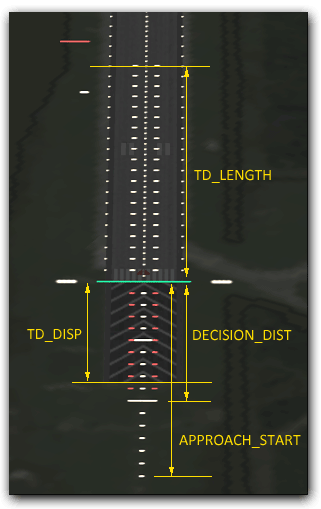
\includegraphics[width=0.5\textwidth]{rwylights.png}}
	\caption{D3D9 runway light parameters}
\end{figure}

\noindent
\textbf{BEACONARRAY}\\
A linear array of illuminated beacons, usable e.g. for taxiway night lighting.

%\begin{table}[H]
	%\centering
	\begin{longtable}{ |p{0.15\textwidth}|p{0.09\textwidth}|p{0.68\textwidth}| }
	\hline\rule{0pt}{2ex}
	\textbf{Parameter} & \textbf{Type} & \textbf{Description}\\
	\hline\rule{0pt}{2ex}
	END1 & Vector & First end point of beacon array in local base coordinates [m]. y-coordinate is elevation above ground.\\
	\hline\rule{0pt}{2ex}
	END2 & Vector & Second end point of beacon array [m].\\
	\hline\rule{0pt}{2ex}
	COUNT & Integer & Number of beacons in the array ($\geq$ 2). Default: 10\\
	\hline\rule{0pt}{2ex}
	SIZE & Float & Size (radius) of each beacon light. Default: 1.0\\
	\hline\rule{0pt}{2ex}
	COL & Float Float Float & Beacon colour (RGB). Range: 0-1 for each value. Default: 1 1 1 (white)\\
	\hline
	\end{longtable}
%\end{table}

\noindent
\textbf{SOLARPLANT}\\
A grid of ground-mounted solar panels, smart enough to align themselves with the Sun. The following parameters are supported:

%\begin{table}[H]
	%\centering
	\begin{longtable}{ |p{0.15\textwidth}|p{0.09\textwidth}|p{0.68\textwidth}| }
	\hline\rule{0pt}{2ex}
	\textbf{Parameter} & \textbf{Type} & \textbf{Description}\\
	\hline\rule{0pt}{2ex}
	POS & Vector & Centre position of the panel grid [m]. Default: 0 0 0\\
	\hline\rule{0pt}{2ex}
	SCALE & Vector & Scaling factor for each panel [m]. Default: 1.0\\
	\hline\rule{0pt}{2ex}
	SPACING & Float Float & Distance between panels in x and z directions [m]. Default: 40 40\\
	\hline\rule{0pt}{2ex}
	GRID & Integer Integer & Grid dimensions in x and z directions [m]. Default: 2 2\\
	\hline\rule{0pt}{2ex}
	ROT & Float & Rotation of plant around vertical axis [deg]. Default: 0\\
	\hline\rule{0pt}{2ex}
	TEX & String [Float Float] & Texture name and u, v scaling factors for panels. Default: no texture\\
	\hline
	\end{longtable}
%\end{table}

\noindent
\textbf{TRAIN1}\\
A monorail-type train on a straight track. The following parameters are supported:

%\begin{table}[H]
	%\centering
	\begin{longtable}{ |p{0.15\textwidth}|p{0.09\textwidth}|p{0.68\textwidth}| }
	\hline\rule{0pt}{2ex}
	\textbf{Parameter} & \textbf{Type} & \textbf{Description}\\
	\hline\rule{0pt}{2ex}
	END1 & Vector & First end point of track [m].\\
	\hline\rule{0pt}{2ex}
	END2 & Vector & Second end point of track [m].\\
	\hline\rule{0pt}{2ex}
	MAXSPEED & Float & Maximum speed of train [m/s]. Default: 30\\
	\hline\rule{0pt}{2ex}
	SLOWZONE & Float & Distance over which the train slows down at the track ends [m]. Default: 100\\
	\hline\rule{0pt}{2ex}
	TEX & String & Texture name\\
	\hline
	\end{longtable}
%\end{table}

\noindent
\textbf{TRAIN2}\\
Suspended train on elevated straight track. The following parameters are supported:

%\begin{table}[H]
	%\centering
	\begin{longtable}{ |p{0.15\textwidth}|p{0.09\textwidth}|p{0.68\textwidth}| }
	\hline\rule{0pt}{2ex}
	\textbf{Parameter} & \textbf{Type} & \textbf{Description}\\
	\hline\rule{0pt}{2ex}
	END1 & Vector & First end point of track [m].\\
	\hline\rule{0pt}{2ex}
	END2 & Vector & Second end point of track [m].\\
	\hline\rule{0pt}{2ex}
	HEIGHT & Float & Elevation of suspension track over ground [m]. Default: 11\\
	\hline\rule{0pt}{2ex}
	MAXSPEED & Float & Maximum speed of train [m/s]. Default: 30\\
	\hline\rule{0pt}{2ex}
	SLOWZONE & Float & Distance over which the train slows down at the track ends [m]. Default: 100\\
	\hline\rule{0pt}{2ex}
	TEX & String & Texture name\\
	\hline
	\end{longtable}
%\end{table}

\noindent
\textbf{LPAD1}\\
An octagonal bordered landing pad. Default diameter 80 m (at scale 1). Landing pads are numbered in the order they appear in the list. This landing pad style can be assigned numbers 1-9, so must be within the first 9 landing pad definitions of the base object list. Orbiter provides a texture map compatible with LPAD1 (Textures\textbackslash Lpad01.dds). Any user-defined texture should adhere to the same layout.

%\begin{table}[H]
	%\centering
	\begin{longtable}{ |p{0.15\textwidth}|p{0.09\textwidth}|p{0.68\textwidth}| }
	\hline\rule{0pt}{2ex}
	\textbf{Parameter} & \textbf{Type} & \textbf{Description}\\
	\hline\rule{0pt}{2ex}
	POS & Vector & Pad centre coordinates in local base frame [m].\\
	\hline\rule{0pt}{2ex}
	SCALE & Float & Scaling factor. Default: 1\\
	\hline\rule{0pt}{2ex}
	ROT & Float & Rotation around vertical axis [deg]. Default: 0\\
	\hline\rule{0pt}{2ex}
	TEX & String & Texture name. Default: no texture\\
	\hline\rule{0pt}{2ex}
	NAV & Float & Frequency of VTOL nav transmitter [MHz] (range 85.0-140.0). Default: no transmitter\\
	\hline
	\end{longtable}
%\end{table}

\noindent
\textbf{LPAD2}\\
A square landing pad. Default size 80 m (at scale 1). Landing pads are numbered in the order they appear in the list. This landing pad style can be assigned numbers 1-99, so must be within the first 99 landing pad definitions of the base object list. Orbiter provides a texture map compatible with LPAD2 (Textures\textbackslash Lpad02.dds). Any user-defined texture should adhere to the same layout.

%\begin{table}[H]
	%\centering
	\begin{longtable}{ |p{0.15\textwidth}|p{0.09\textwidth}|p{0.68\textwidth}| }
	\hline\rule{0pt}{2ex}
	\textbf{Parameter} & \textbf{Type} & \textbf{Description}\\
	\hline\rule{0pt}{2ex}
	POS & Vector & Pad centre coordinates in local base frame [m].\\
	\hline\rule{0pt}{2ex}
	SCALE & Float & Scaling factor. Default: 1\\
	\hline\rule{0pt}{2ex}
	ROT & Float & Rotation around vertical axis [deg]. Default: 0\\
	\hline\rule{0pt}{2ex}
	TEX & String & Texture name. Default: no texture\\
	\hline\rule{0pt}{2ex}
	NAV & Float & Frequency of VTOL nav transmitter [MHz] (range 85.0-140.0). Default: no transmitter\\
	\hline
	\end{longtable}
%\end{table}

\noindent
\textbf{LPAD2A}\\
Similar to LPAD2, but uses a different layout for the texture map, providing a higher resolution at the same texture size. Orbiter provides a texture map compatible with LPAD2A (Textures\textbackslash Lpad02a.dds). Any user-defined texture should adhere to the same layout. The supported parameters are the same as for LPAD2.\\


\noindent
\textbf{MESH}\\
Generic mesh for custom objects. Mesh files must be in Orbiter mesh file format (see section \ref{sec:mesh_file})

%\begin{table}[H]
	%\centering
	\begin{longtable}{ |p{0.22\textwidth}|p{0.09\textwidth}|p{0.65\textwidth}| }
	\hline\rule{0pt}{2ex}
	\textbf{Parameter} & \textbf{Type} & \textbf{Description}\\
	\hline\rule{0pt}{2ex}
	FILE & Float & Mesh file name (without path and extension). Mesh files must be located in the mesh subdirectory (as defined in the main config file)\\
	\hline\rule{0pt}{2ex}
	POS & Float & Position of the mesh origin in local base coordinates [m]\\
	\hline\rule{0pt}{2ex}
	SCALE & Float & Scaling factors in along the 3 axes (height in y). Default: 1 1 1\\
	\hline\rule{0pt}{2ex}
	ROT & Float & Rotation around the vertical axis [deg]. Default: 0\\
	\hline\rule{0pt}{2ex}
	TEX & Float & Texture name. Default: none\\
	\hline\rule{0pt}{2ex}
	WRAPTOSURFACE & Flag & Wrap mesh vertices to the planet surface (e.g. taxiways and similar)\\
	\hline\rule{0pt}{2ex}
	SHADOW & Flag & Render the shadow cast on the ground by the object (cannot be used together with OWNSHADOW)\\
	\hline\rule{0pt}{2ex}
	OWNSHADOW & Flag & Use group shadow flags in mesh file to set shadows for individual mesh groups (cannot be used together with SHADOW)\\
	\hline\rule{0pt}{2ex}
	UNDERSHADOWS & Flag & Object can be covered by shadows cast on the ground by other objects (e.g. roads, landing pads, etc.). Default: object not covered by ground shadows\\
	\hline\rule{0pt}{2ex}
	OWNMATERIAL & Flag & Use materials and textures defined in the mesh file. This overrides the TEX entry.\\
	\hline\rule{0pt}{2ex}
	LPAD & Flag & Object is a landing pad\\
	\hline\rule{0pt}{2ex}
	PRELOAD & Flag & Mesh should be loaded at program start. This can reduce disc activity during the simulation, but increases main memory usage. Default: load only when used.\\
	\hline
	\end{longtable}
%\end{table}

\noindent
Notes:

\begin{itemize}
\item If the mesh only uses a single texture it is more efficient to specify it via the TEX entry instead of defining it in the mesh and using the OWNMATERIAL flag, because Orbiter can merge objects with the same TEX entries for improved performance.
\item If OWNSHADOW is used, any mesh groups which have bit 0 set in their FLAG entry do not cast shadows, otherwise they do cast shadows (see section \ref{sec:mesh_file}).
\end{itemize}


\subsection{Custom markers}
\label{ssec:custom_markers}
\alertbox{As regards markers for planetary surface features, this section contains information for old-style (pre-Orbiter 2016) marker definitions. These are retained for backward compatibility. For new, quadtree-based marker definitions, see section \ref{sssec:label_tile_format}.}

\noindent
Labels can be defined to mark objects on the celestial sphere (e.g. bright stars, navigation stars, nebulae, etc.) or on planetary surfaces (legacy) to locate natural landmarks, points of interest, historic landing sites, navigational aids, etc.\\
The user can display these markers during the simulation with the Visual helpers option (\keystroke{F9} or \Alt\keystroke{F9}).\\
By default, all files for celestial and planetary surface markers are placed in a subdirectory\\
\indent .\textbackslash Config\textbackslash <\textit{name}>\textbackslash Marker\\
where <\textit{name}> is the name of the planetary system (for celestial markers) or the celestial body (for legacy surface markers) they are referring to. A different location for marker files can be specified with the MarkerPath option in the planetary system's or planet's configuration file (see sections \ref{ssec:planetery_sys} and \ref{ssec:planets}). Marker files are text files with extension .mkr. Multiple files can be defined for a single planet or planetary system, which the user can turn on and off individually. The format is

\begin{lstlisting}[language=OSFS]
BEGIN_HEADER
	InitialState [on|off]
	ShapeIdx [0 - 6]
	ColourIdx [0 - 5]
	Size [0.1 - 2]
	DistanceFactor [1e-5 - 1e3]
	Frame [celestial|ecliptic]
END_HEADER
BEGIN_DATA
	<lng> <lat> : <label> [: <label>]
	<lng> <lat> : <label> [: <label>]
	...
\end{lstlisting}

\noindent
The header section contains some configuration options:

\begin{itemize}
\item InitialState $\Rightarrow$ defines if the labels are initially visible when the user activates surface or celestial markers in the \textit{Visual helpers} dialog. The user can turn lists on and off individually during the simulation. The default is off.
\item ShapeIdx $\Rightarrow$ is an integer between 0 and 6 defining the shape of the label markers:

%\begin{table}[H]
	%\centering
	\begin{longtable}{ |p{0.04\textwidth}|p{0.04\textwidth}|p{0.2\textwidth}| }
	\hline\rule{0pt}{2ex}
	0 & $\Box$ & box (default)\\
	\hline\rule{0pt}{2ex}
	1 & $\bigcirc$ & circle\\
	\hline\rule{0pt}{2ex}
	2 & $\Diamond$ & diamond\\
	\hline\rule{0pt}{2ex}
	3 & $\nabla$ & nabla\\
	\hline\rule{0pt}{2ex}
	4 & $\Delta$ & delta\\
	\hline\rule{0pt}{2ex}
	5 & + & crosshair\\
	\hline\rule{0pt}{2ex}
	6 & $\times$ & rotated crosshair\\
	\hline
	\end{longtable}
%\end{table}

\item ColourIdx $\Rightarrow$ is an integer between 0 and 5 defining the colour of the labels:

%\begin{table}[H]
	%\centering
	\begin{longtable}{ |p{0.04\textwidth}|p{0.04\textwidth}|p{0.2\textwidth}| }
	\hline\rule{0pt}{2ex}
	0 & \cellcolor[HTML]{FFFF00} & yellow\\
	\hline\rule{0pt}{2ex}
	1 & \cellcolor[HTML]{00FFFF} & cyan (default)\\
	\hline\rule{0pt}{2ex}
	2 & \cellcolor[HTML]{FF3F3F} & red\\
	\hline\rule{0pt}{2ex}
	3 & \cellcolor[HTML]{FF00FF} & purple\\
	\hline\rule{0pt}{2ex}
	4 & \cellcolor[HTML]{3FFF3F} & green\\
	\hline\rule{0pt}{2ex}
	5 & \cellcolor[HTML]{007FFF} & blue\\
	\hline
	\end{longtable}
%\end{table}

\item Size $\Rightarrow$ scales the marker size. Default: 1.0
\item DistanceFactor $\Rightarrow$ resets the distance up to which camera distance the markers are displayed. Default: 1.0
\item Frame $\Rightarrow$ (used for celestial markers only) defines the reference to which the coordinates in the list refer:

\begin{itemize}
\item ecliptic: coordinates are ecliptic longitude and latitude
\item celestial: coordinates are right ascension and declination of J2000 equator and equinox
\end{itemize}

\end{itemize}

\noindent
Each item in the header section is optional. If missing, the default value is substituted. The header can also be omitted altogether, in which case the BEGIN\_DATA tag is also not required.\\
In the data section, each line defines a label. It consists of equatorial position: longitude [deg], with eastern longitudes positive and western longitudes negative, latitude [deg], with northern latitudes positive and southern latitudes negative, and one or two label strings to be displayed above and below the marker.

\end{document}
